
%!TEX root = ../thesis.tex
%*******************************************************************************
%****************************** Third Chapter **********************************
%*******************************************************************************
\chapter{Simulating SBND}
\label{ChapterSim}

% **************************** Define Graphics Path **************************
\ifpdf
    \graphicspath{{Chapter6/Figs/Raster/}{Chapter6/Figs/PDF/}{Chapter6/Figs/}}
\else
    \graphicspath{{Chapter6/Figs/Vector/}{Chapter6/Figs/}}
\fi

%********************************** %Opening  **************************************

%Modern physics experiments and MC
Many modern particle physics experiments heavily rely on simulations, of which many employs the Monte Carlo (MC) technique by random sampling from a predefined distributions.
Simulation is particularly useful for an early stage experiment like SBND where the detector is not yet operational to record data.
Simulation enables for study of the physics capabilities of the detector as well as to develop reconstruction and analysis tools in preparation for data.
The search for HNLs at SBND presented here is an exploration of the detector physics capabilities in the BSM regime, given that the detector timing resolution is able to achieve nanosecond resolution.

The following chapter provides a detailed description of the simulation workflow at SBND to output simulated product that ideally represents real data.
The chapter begins with an overview of the workflow in Sec. \ref{sec:overview_sim}.
Meanwhile, Sec. \ref{sec:gen_mevprtl} includes the details of the generator employed to generate a signal event of HNLs and Sec. \ref{sec:gen_sm} provides the summary of the generator used to generate background events from SM neutrinos and cosmic muons.
Furthermore, details in Sec. \ref{sec:gen_response} follows the simulation of energy deposition as the particle propagates through the detector, and consequently the simulation of the detector response to the energy.
Finally, some concluding remarks are provided in Sec. \ref{sec:sim_concluding_remarks}.

\newpage

%********************************** %First Section  **************************************
\section{Overview of Simulating SBND}
\label{sec:overview_sim}

Similar to many other LArTPCs, the software framework for simulation, reconstruction and analysis of SBND is provided by the LArSoft framework \cite{larsoft}.
The framework was built for neutrino experiments sharing the same common feature of having LArTPCs, while still allowing for detector-specific customisation.
This enables easy sharing software tools across many collaborations including ArgoNeuT, MicroBooNE, ICARUS, SBND and DUNE.
For example, the generator used to simulate HNLs, to be discussed in the next section, has been developed and shared across the SBND and ICARUS collaboration.

%Describe the overall workflow
The simulation workflow of SBND under the LArSoft framework is depicted in Fig. \ref{fig:Sim_Workflow}.
The process begins with a generator to produce primary particles that enter the detector, shown by the purple box.
The primary particles can be neutrinos, cosmic muons or BSM particles depending on the type of generator.
The propagation of the primary particle inside and outside the detector, and the resulting energy deposition is simulated using the Geant4 tool kit \cite{geant4}, shown by the green boxes.
For interactions inside the detector, the charge and light yield is calculated from the energy deposition.
The number of ionisation electrons from the charge yield are propagated through the detector to the wire planes using Wirecell tool kit \cite{wirecell}, shown by the red boxes.
The number of scintillation photons from the light yield are propagated to the photodetectors using a combination of semi-analytical model and light libray \cite{sbnd_pds_paper}, shown by the blue boxes.
For interactions outside of the detector, only the energy depositions within the CRT strips are converted converted into light yield, shown by the orange box.
The detector response is then simulated for each detector subsystem.
By the end of this stage, the outputs from each detection subsystem ideally represent real data.

\begin{figure}[htbp!] 
\centering    
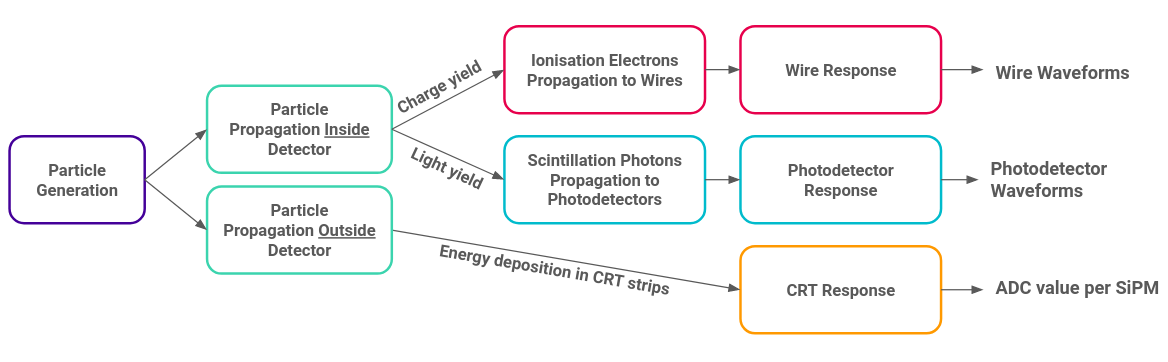
\includegraphics[width=1.0\textwidth]{Sim_Workflow}
\caption[Sim_Workflow]{
Overview of the workflow to simulate the SBND detector.
}
\label{fig:Sim_Workflow}
\end{figure}

\section{HNL Generator: MeVPrtl}
\label{sec:gen_mevprtl}

%MeVPrtl Workflow
HNLs are generated using the MeVPrtl generator \cite{}, which is joint effort by ICARUS and SBND collaborators towards a sharing BSM generator.
MeVPrtl was developed as a modular generator, allowing for easy adaptations for different beam sources and detectors, as well as direct interface with the existing LArSoft framework.
The workflow of the MeVPrtl is broken down into 4 stages, as illustrated in Fig. \ref{fig:MeVPrtl_Workflow}.
The generator begins with taking an input of meson fluxes, representing the particles produced from a beam source.
It then simulates the meson decaying to a BSM particle, which is propagated to the detector and decays back into a SM observable.
There are several BSM models already implemented in the MeVPrtl generator, including HNLs, Higgs portal scalars \cite{} and heavy QCD axions \cite{}.


\begin{figure}[htbp!] 
\centering    
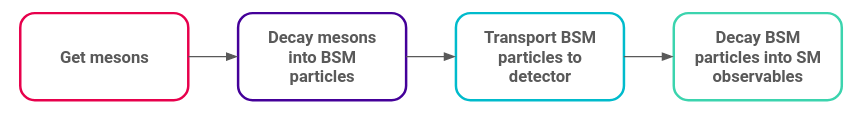
\includegraphics[width=1.0\textwidth]{MeVPrtl_Workflow}
\caption[MeVPrtl_Workflow]{
Overview of the workflow of the MeVPrtl generator.
}
\label{fig:MeVPrtl_Workflow}
\end{figure}

%Each stage validation
For the purpose of generating HNLs coming from the BNB, the generator begins with sampling the charged kaons $K^{+}$ fluxes of the BNB.
Instead of decaying into a SM neutrino, the kaons decay either in-flight or at rest into a HNL, with branching ratio defined by Eq. \ref{eq:kaon_decay_hnl}.
The daughter HNL and lepton are simulated from a two-body decay at rest in the centre of mass frame of the kaon, and then boosted to the parent's lab frame by Lorentz boost.
Due to the HNL having mass, the HNL has less transverse momentum than SM neutrinos and therefore more collimated, travelling preferably to the parent kaon direction.
The Lorentz boost can flip the directions of HNLs from low energy kaons that are originally emitted backwards \cite{DavidePhD}.
The HNL is then propagated to detector by the ray tracing method, which forces the HNL to hit the SBND detector by picking a direction that impinges the particle at the detector front face.
The probability for enforcing the detector intersection is also computed.
Example angular distribution in lab frame of the parent kaons and the HNLs that arrive at the SBND detector is shown in Fig. \ref{fig:kaon_hnl_angle2beam}.
For plotting completeness, the selected parent kaons have energies peaking approximately $0.5\sim1$ GeV, and evenly distributed in the angle with respect to the beam direction, as shown in Fig. \ref{fig:kaon_angle2beam}.
The resulting HNLs of mass 240 MeV and their angles to the beam direction is shown in Fig. \ref{fig:hnl_angle2beam}.
This demonstrates that the acceptance angle of the HNLs to hit the SBND detector is very small ($\theta < 5^\circ$), such that only very forward-going HNLs are most likely to intersect detector.

\begin{figure}[tbp!]
        \centering
        \begin{subfigure}[b]{0.495\textwidth}
            \centering
            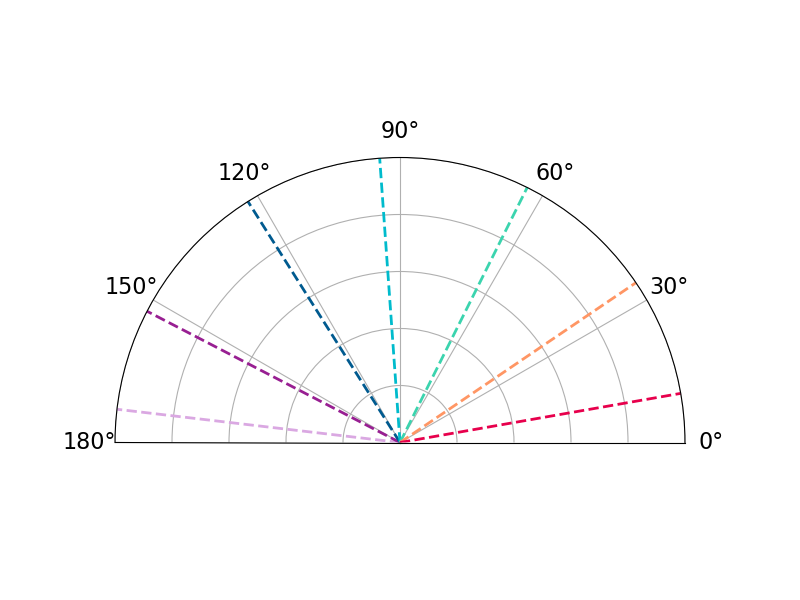
\includegraphics[width=\textwidth]{kaon_angle}
            \caption{Kaons}%
            \label{fig:kaon_angle2beam}
        \end{subfigure}
        \hfill
        \begin{subfigure}[b]{0.495\textwidth}  
            \centering 
            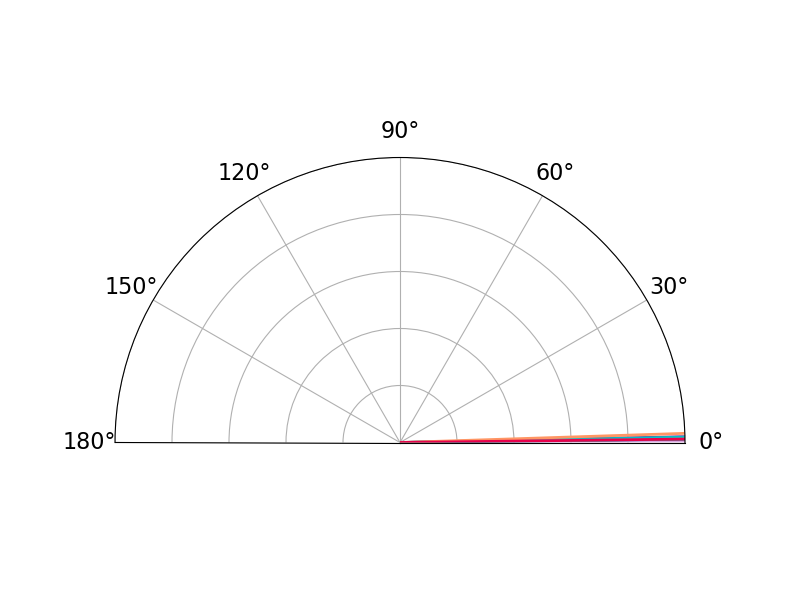
\includegraphics[width=\textwidth]{hnl_angle}
            \caption{HNLs}%
            \label{fig:hnl_angle2beam}
        \end{subfigure}
        \caption[kaon_hnl_angle2beam]{Example distributions of angle to the beam direction, for the parent kaons and for the resulting HNLs that arrive at the detector.}
        \label{fig:kaon_hnl_angle2beam}
\end{figure}

The resulting fluxes of HNL arriving at the SBND detector is depicted in Fig. \ref{fig:HNL_Energy_Spectrum} for the mass range between 140 and 240 MeV.
The fluxes are normalised to the same mixing angle $|U_{\mu4}|^{2} = 1 \times 10^{-7}$ and 3 years of data taking, equivalent to $1 \times 10^{21}$ POT.
At the same mixing angle, the expected HNL rate decreases with lower mass since the branching  ratio of $N \rightarrow \nu\pi^0$ decreases with lower mass, as previously shown in Fig. \ref{fig:branchingRatio}.
Since the $K^{+}$ flux peaks around 0.5 GeV and decreases at higher energy, as previously shown in Fig. \ref{fig:BNB_Meson_Flux}, the HNL fluxes also mainly concentrate in the low energy region, and substantially decrease at higher energy. 
Moreover, across the HNL mass range, there are more energetic HNLs at a lower mass than at a higher mass.
This is due to HNLs coming from a kaon decay and therefore, the lighter the HNL mass, the more kinetic energy is available.
Finally, all the HNL fluxes have a sharp peak near zero, corresponding the HNLs resulting from kaons decay at rest.

Once arrive at the detector, the HNL decays back into the SM observables.
For example of the $\nu\pi^{0}$ final state, the decay width is defined by Eq. \ref{eq:pi0}.
\begin{figure}[tbp!] 
\centering    
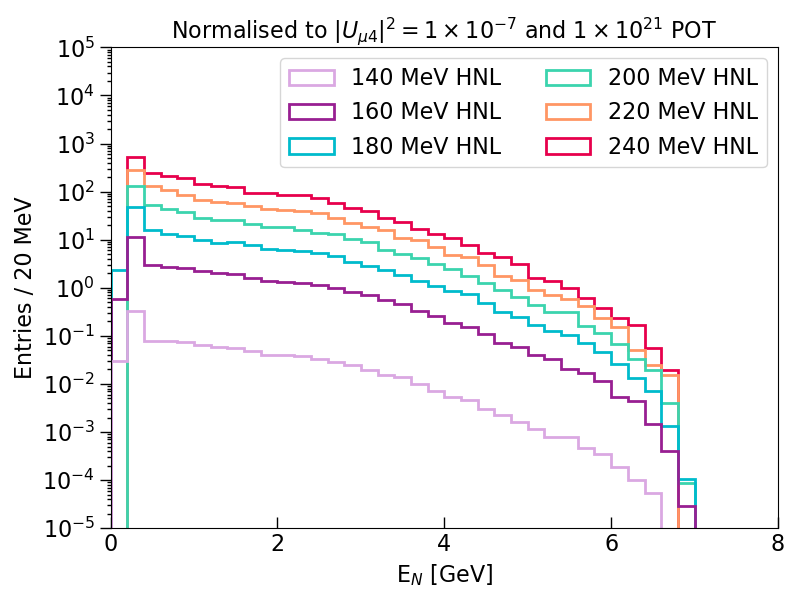
\includegraphics[width=0.65\textwidth]{HNL_Energy_Spectrum}
\caption[HNL_Energy_Spectrum]{
Simulated HNL fluxes for mass ranging from 140 to 240 MeV, normalised to the mixing angle $|U_{\mu4}|^{2} = 1 \times 10^{-7}$ and $1 \times 10^{21}$ POT.
}
\label{fig:HNL_Energy_Spectrum}

%\end{figure}
%\begin{figure}[bp!]

        \centering
        \begin{subfigure}[b]{0.495\textwidth}
            \centering
            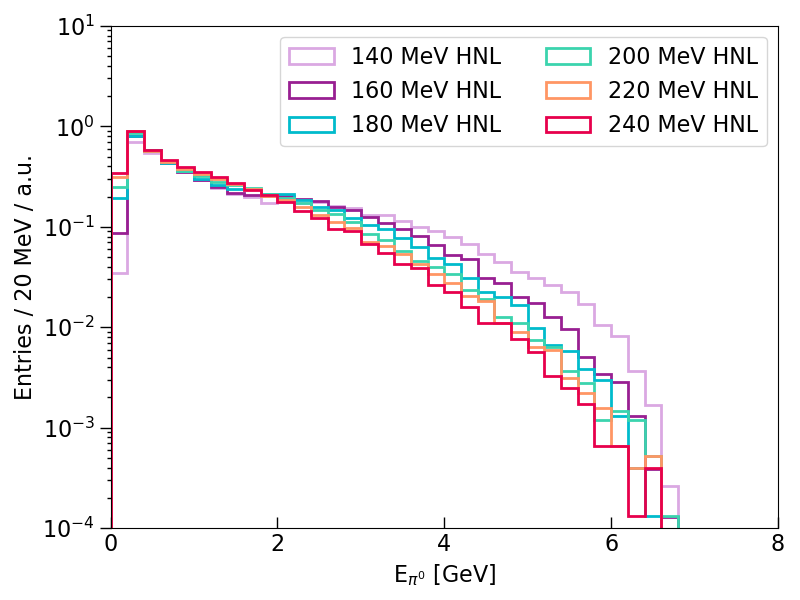
\includegraphics[width=\textwidth]{pi0_energy}
            \caption{Energy Distribution}%
            %\label{fig:kaon_angle2beam}
        \end{subfigure}
        \hfill
        \begin{subfigure}[b]{0.495\textwidth}  
            \centering 
            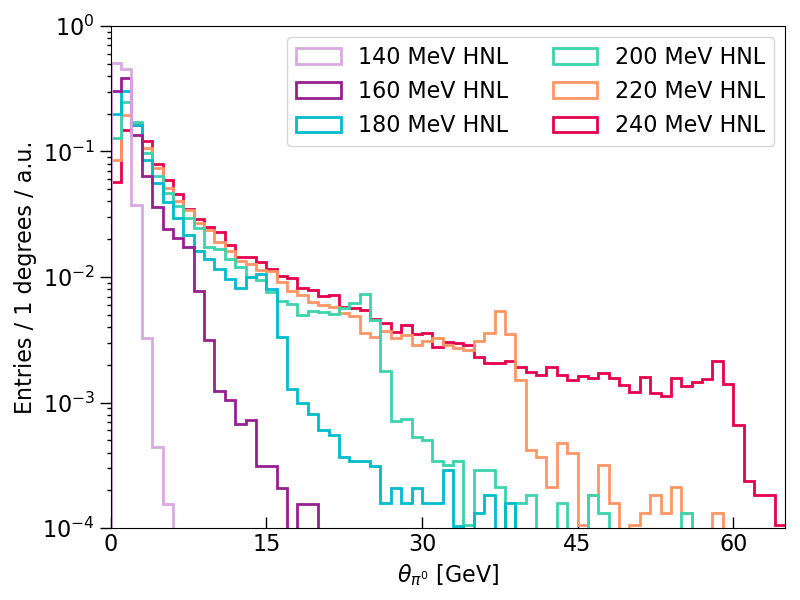
\includegraphics[width=\textwidth]{pi0_angle2Beam}
            \caption{Angle to the Beam Direction Distribution}%
            %\label{fig:hnl_angle2beam}
        \end{subfigure}
        \caption[pi0_distribution]{Kinematic distributions for neutral pions resulting from HNLs decaying inside the SBND detector.}
        \label{fig:pi0_distribution}
\end{figure}
The kinematics of the decay products is simulated for a HNL isotropically decays in its rest frame, and the boosted to its lab frame by Lorentz boost.
Since the parent HNL is very forward-going, the daughter $\pi^0$ is also forward-going, with momenta dependency on the mass of the parent HNL. 
Fig \ref{fig:pi0_distribution} shows the energy and angle to the beam distributions for the daughter $\pi^0$.
The plots are area-normalised for comparison across the mass range of the parent HNL from 140 to 240 MeV. 
The energy distribution of the $\pi^0$ decreases as the HNL mass increases since heavier HNLs are less energetic and therefore, less energy available for the $\pi^0$.
As a result, the angle to the beam of $\pi^0$ also widens with heavier HNL.
Even so, at the HNL mass of 240 MeV, the $\pi^0$ is still collimated with angular distribution dominate in the region $< 30^\circ$. 
Therefore, the di-photon showers from the HNL-originated $\pi^0$ are expected to be more forward-going with respect to the those originate from SM neutrinos.
Finally, the peak in the angular distribution come from low energy HNL resulting from kaons decay at rest.

%Timing
One key motivation of the HNL search is the timing delay between a HNL compared to a SM neutrino, due to a HNL being massive compared to a SM neutrino.
The total time of flight for a HNL or a SM neutrino from the BNB to the SBND detector is illustrated in Fig. \ref{fig:tof_beam_to_detector}.
The first component is the spill time of the protons from the Booster synchrotron, $t_{spill}$, which is the same for both a HNL and a SM neutrino.
The structure of $t_{spill}$ is the beam bucket structure made up of 81 Gaussian buckets with a width of 1.308 ns and a spacing of 19 ns, which was previously detailed in Sec. \ref{sec4BNB}.   

\begin{figure}[htbp!] 
\centering    
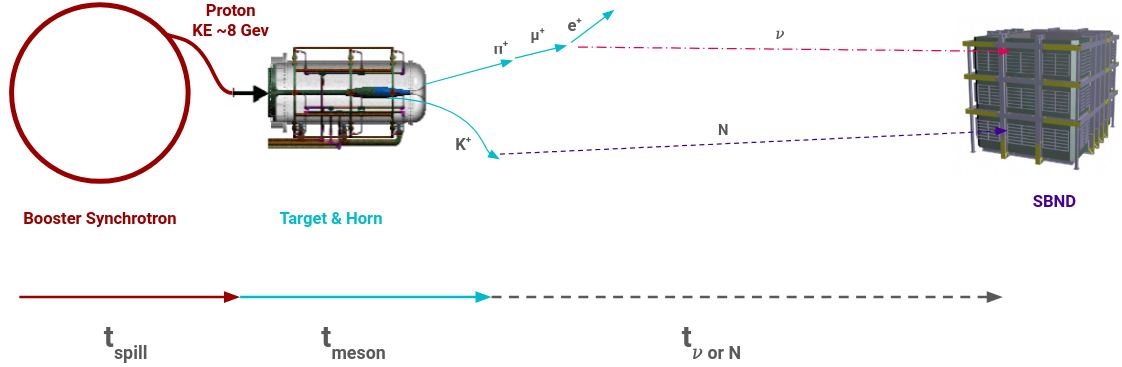
\includegraphics[width=1.0\textwidth]{tof_beam_to_detector}
\caption[tof_beam_to_detector]{
Diagram of the time of flight for a SM neutrino or a HNL, starting from the Booster synchrotron until the interaction time inside the SBND detector.
}
\label{fig:tof_beam_to_detector}
\end{figure}

The second component is the time of the secondary mesons, $t_{meson}$, which is the time from when the mesons are produced until they decay into a HNL or a SM neutrino.
This time accounts for the time the mesons travelling down the decay pipe, and might interact, re-scatter or decay into other mesons.
In the case of the HNL, $t_{meson}$ is primarily the time of flight of the charged kaons $K^+$ before decaying into a HNL.
On the other hands, the SM neutrinos comes from a variety of parent mesons $t_{meson}$, previously listed in Fig. \ref{fig:BNB_neutrino_flux}.
In both cases, $t_{meson}$ introduces some smearing to the nanosecond-bucket structure of $t_{spill}$.

The last component is the time of flight of the SM neutrino or the HNL from the creation point to the interaction point inside the SBND detector.
In the case of the SM neutrinos, since neutrinos are nearly massless, their velocity can be approximated as a speed of light. 
Then, the time of flight of the neutrino is  
\begin{equation}
	t_{\nu} = \frac{d_{\nu}}{c}
\end{equation}
where $d_{\nu}$ is the distance of a neutrino from creation to interaction inside the detector.
Meanwhile, HNLs are massive and therefore, travel at a velocity $v_N < c$.
The time of flight of the HNL is
\begin{equation}
	t_{N} = \frac{d_{N}}{v_N}
\end{equation}
where $d_N$ is the distance of a HNL from creation to decay inside the detector.
Additionally, since the energy of the HNL decreases with its mass, the heavier it is, the slower its velocity.
Thus, heavier HNLs arrive even later compared to lighter HNLs.

The advantage the MeVPrtl generator is the consistency of simulating the time of flight described above, for a HNL using the MeVPrtl generator and for a SM neutrino using the GENIE generator.
Fig. \ref{fig:full_beam} shows the arrival time of the SM neutrinos and 240 MeV HNLs at the front face of the SBND detector, recovering the beam spill structure of the BNB.
The plot is area-normalised to enable the comparison between the two particles. 
Since the SM neutrinos travel nearly at the speed of light, less smearing is introduced and the timing distribution shows sharp Gaussian peaks.
\begin{figure}[bp!] 
\centering    
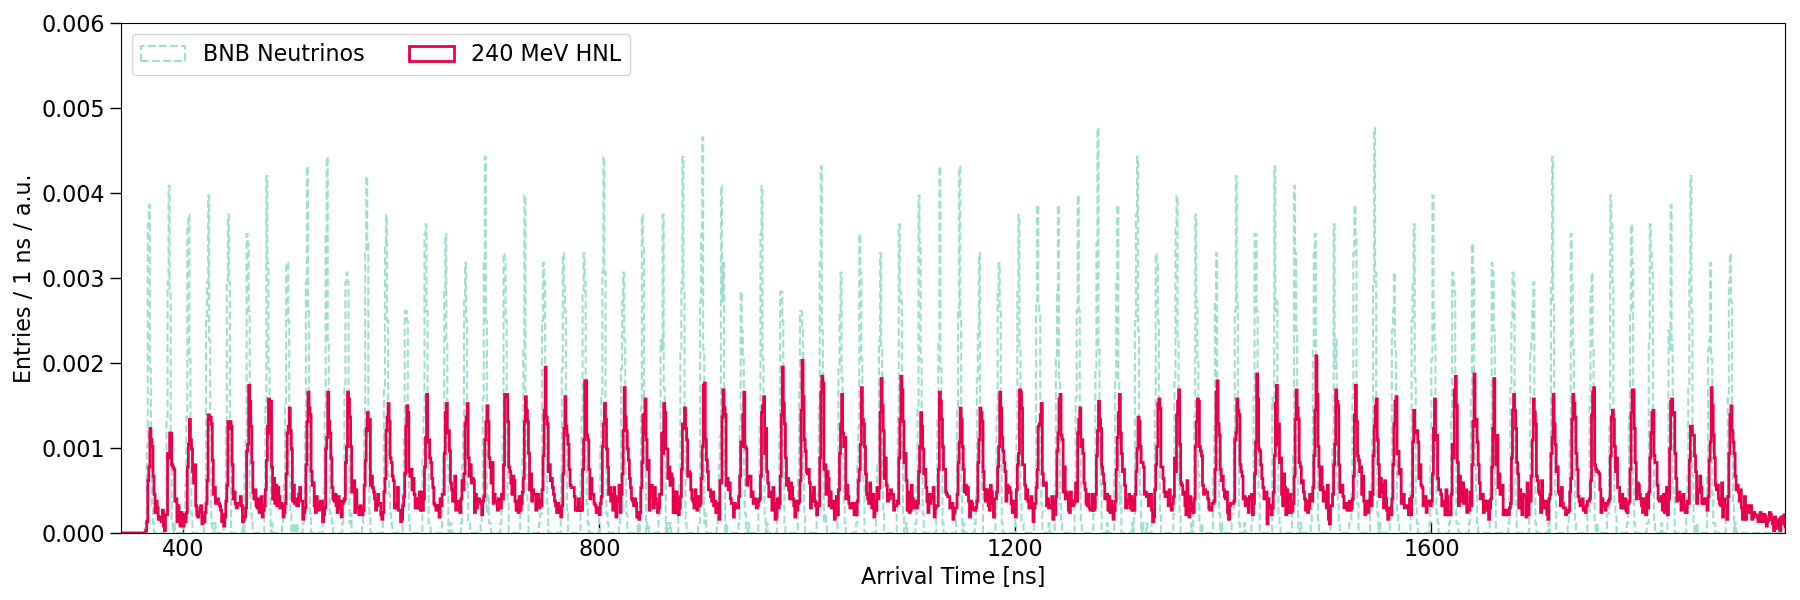
\includegraphics[width=1.0\textwidth]{full_beam}
\caption[full_beam]{
Distribution of the arrival time at the front face of the SBND detector for SM neutrinos simulated by the GENIE generator and for HNLs simulated by the MeVPrtl. 
}
\label{fig:full_beam}
\end{figure}
On the other hands, the HNLs travel slower and therefore, add additional smearing and delay tails to the Gaussian peaks.
For clarity, 81 Gaussian peaks are overlay into one by taking the modulus of 19 ns, as shown in Fig. \ref{fig:beam_modulus}.
The timing distribution of the HNLs show a clear distinction to the SM neutrinos, where delay tails on either sides of the Gaussian peak can be seen.
Across the mass range of HNL from 140 to 240 MeV, the delay tails however do not increase significantly with mass. 

\begin{figure}[htbp!] 
\centering    
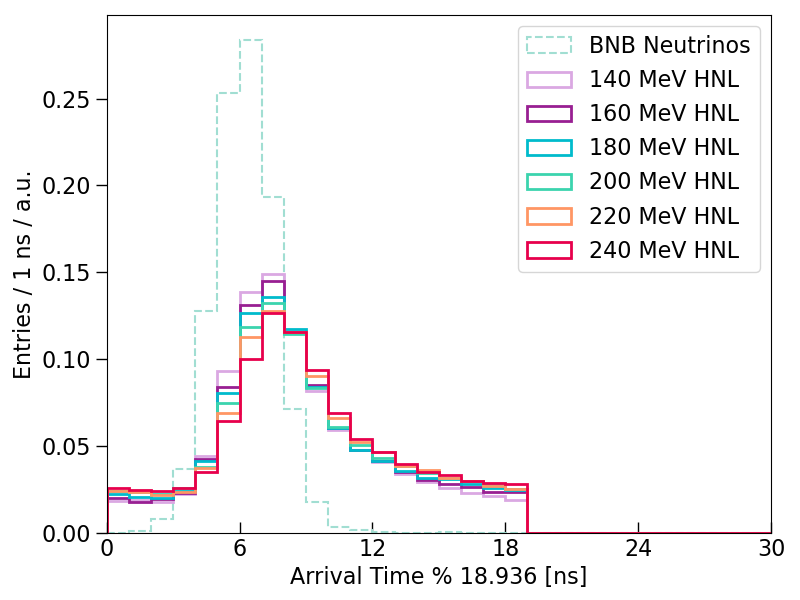
\includegraphics[width=0.65\textwidth]{beam_modulus}
\caption[beam_modulus]{
Modulus of the of arrival time distribution of SM neutrinos and HNLs with mass ranging from 140 to 240 MeV. 
}
\label{fig:beam_modulus}
\end{figure}

\section{Other SM Generators}
\label{sec:gen_sm}

\subsection{Neutrino Generator: GENIE}
\label{sec:gen_genie}

%Overview of GENIE

%What kind of tune are being used

SM neutrino interactions are generated by the GENIE generator \cite{genie}, which provides a selection of theoretical and empirical models for different physic process.
These models can be combined into a \textit{tune} by comparing predictions to data from neutrino and electron scattering experiments.
The SBND collaboration is planning to use a tune that was specifically developed to serve as a baseline model for the SBN and DUNE oscillation analysis.
Details for the basis of the tune can be found in Table 1 in Ref. \cite{genie_tune}, with ongoing developments on the choice of models documented in Ref. \cite{genie_tune_github}.  

In general, GENIE first selects a nuclear model that describes the momenta and potential energy of the nucleons to model nuclear effects.
Then, the neutrino flux and the integrated cross section model are used to compute the probability if a neutrino interaction occurs.
The differential cross section is then used to determine the type of neutrino interaction and the kinematic range.
The neutrino interaction types include Quasi-Elastic (QE), Baryonic Resonant Scattering (RES), Coherent Scattering (COH), Deep Inelastic Scattering and $\nu$-e elastic scattering.
DIS interaction can additionally produce hadrons within the nuclei, of which these hadrons can propagate through the nucleus and modify the observed kinematics.
Thus, the choice of Final State Interaction (FSI) model is also crucially important for predicting the observable topology of neutrino interactions since argon is a heavy nuclear target.

In addition to the tune, the GENIE generator also provides a re-weighting scheme to evaluate the systematic uncertainties for a model chosen in the tune.
Due to the scarcity of neutrino interaction data, particularly for $\nu-Ar$ interaction, the uncertainties in cross section modelling tend to be large, and can hamper the capabilities of the HNL sensitivity.  
The neutrino interaction re-weighting scheme, and the resulting systematics uncertainties impact on the HNL search will be discussed in details in Sec. \ref{}.


GENIE simulates neutrino interactions occurring both inside and outside of the detector volume, with boundary defined in Fig. \ref{fig:Rockbox_Volume}.  
All interactions occurring inside the detector volume are strictly kept.
Outside of the detector, a buffer volume is defined as 5 m surrounding the detector volume.
An additional Rockbox volume is defined by extending the buffer volume backwards in the beam direction ($z$-axis) up to 15 m in front of the buffer volume.
Both these volumes are referred to together as the \textit{Rockbox} volume in this thesis.
Neutrino interactions within this volume are kept, whose products can potentially deposit energy in the detector.
These interactions are referred to as \textit{dirt} neutrinos, and constitute to a significant background to the HNL search.
The background rejection of dirt neutrinos will be covered in Sec. \ref{}.

\begin{figure}[htbp!] 
\centering    
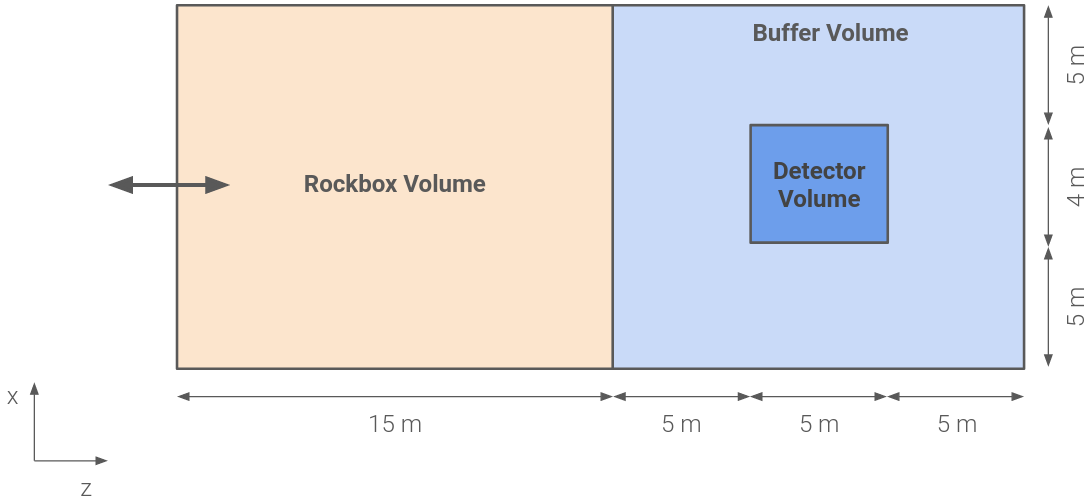
\includegraphics[width=0.85\textwidth]{Rockbox_Volume}
\caption[Rockbox_Volume]{
Diagram showing the volume boundary defined by the GENIE generator to simulate neutrino interactions occurring inside and outside of the detector volume. 
}
\label{fig:Rockbox_Volume}
\end{figure}

\subsection{Cosmic Generator: CORSIKA}
\label{sec:gen_corsika}

%how corsika generator works
Cosmic interactions are simulated using the CORSIKA generator \cite{corsika}.
The generation begins with generating high energy primary particles incident in the Earth's atmosphere, of which only primary protons are kept due to better agreement with MicroBooNE data \cite{}. 
The primaries are then propagated through the atmosphere, interacting with the air to produce secondary decays until reaching the Earth's surface.
Within the SBND simulation workflow, this surface is specified to be just above the roof of the detector building.
The surviving particles are then propagated to the SBND detector.

%Why cosmic simulation is important
From a triggering perspective, there are two types of comic muons as follows 
\begin{itemize}
	\item\textbf{In-time} cosmic muon crosses the detector at the same as a neutrino is present inside the detector, such that the muon is \textit{inside} the beam spill window. The cosmic muon then produces enough light to induce a beam trigger similar to a neutrino.
	\item\textbf{Out-of-time} cosmic muons occurs regardless of the trigger conditions. The muon crosses the detector \textit{outside} the beam spill window, but within the readout window.
\end{itemize}
However, triggering is currently not being simulated in the workflow. 
Only timing requirement is simulated to keep only cosmic muons occurring within the readout window.
Therefore, the simulation does not accurately reflect the cosmic rate once factoring triggering conditions and comparison to data is necessary. 

Being a surface level detector, it is vitally important to understand the cosmic background at SBND due to the exposure to a high cosmic rate.
Once SBND is operational, a particularly useful measurement is the rate of cosmic muons that would cause a beam trigger, however, in absence of the beam.
This is equivalent to measure the rate of cosmic muons that produce sufficient energy inside the detector to mimic a neutrino interaction.
This measurement allows for validation against the CORSIKA generator sampling of the cosmic topology and kinematic distribution. 
Moreover, it also provides an expected cosmic rate given a triggering condition, which can be subsequently added in the simulation workflow to better constrain the cosmic background.

\section{Particle Propagation and Detector Response Simulation}
\label{sec:gen_response}

\subsection{Particle Propagation Simulation}
\label{sec:gen_g4}

Once a particle is simulated inside the detector, it is propagated through the detector using the Geant4 tool kit \cite{geant4}.
Geant4 propagates the particle by each step $dx$, where the step length is randomised and capped at 0.3 mm (one order of magnitude less than the wire pitch).
At each step, physics processes are applied to the particle, such as energy deposition, interaction, decay and so on.
The step propagation also accounts for the electric field distortion due to space charge effects, given that the SBND detector is overground and has a high exposure to cosmic.

The main physics process is energy deposition in the detector is ionisation by charged particles.
Similarly to the theory detailed in Sec. \ref{sec3:creation}, the Geant4 tool kit simulates the ionisation process following the Bethe-Bloch formalism tuned to data \cite{geant4_ions}.
The number of ionisation electrons and scintillation photons from the deposited energy are computed using the ModBox recombination model with ArgoNeuT parameters \cite{argoneut_recomb}, and the charge-light anti-correlation from Eq. \ref{eq:Q} and \ref{eq:L}. 
Further discussion about the simulation of recombination, and the impacts of delta ray fluctuations on recombination will be detailed in Sec. \ref{sec7:delta}.
The result from the Geant4 tool kit is a complete set of charge and light yield along the primary particle trajectories through the detector, and the hierarchy of the daughter particles produced from the primary.
The propagation of the charge and light yield to the corresponding detection subsystem are then simulated, to be covered in the upcoming section.

\subsection{Wire Response}

The simulation of the ionisation electrons drifting to the wire planes are done by the WireCell tool kit \cite{wirecell}.
The simulation transports the electrons, and introduces smearing due to detector effects for transporting electrons though liquid argon under an electric field, which is previously discussed in Sec. \ref{sec:edrift}.
This includes charge attenuation due to impurities, smearing of the electron deposition in timing and spatial dimensions due to longitudinal diffusion, transverse diffusion and space charge effect combined.

Once the electrons arrive at the wire plane, a convolution of the field response and the electronic response is performed.
The field response describes the current induced on wires due to ionisation electrons drifting past the induction planes.
Meanwhile the electronic response describes amplification and shaping by pre-amplifiers of wires.
The response functions are in 2-dimensions, one dimension is in time and the other is in wire.
This is to account for long range charge induction effects on wire signal shapes.
A digitisation step is then applied to produce ADC-level, time-domain waveform for each wire channel.
The waveform is parameterised by the ADC resolution, voltage range and baseline specification of the wire readouts. 
Finally, inherent electronics noise is added to the waveform to better match to observed data.
The output simulated waveforms at this stage ideally represent real data waveforms record by the wire readouts, therefore from this point onwards, Monte Carlo and data waveforms should.

\subsection{PDS Response}

The simulation of the scintillation photons to the optical detectors, including the transport effects previously detailed in Sec. \ref{sec:photonprop}, are simulated using a combination of semi-analytical model described in Ref. \cite{}, and optical library model available in LArSoft \cite{}.
The choice of which model to use depends on the location of the photon production.
The semi-analytical model is used for those produced inside the active volume of the SBND detector, whilst the optical library model is used to those originate outside of this volume.

The semi-analytical model calculates on-the-flight the geometrical aperture for each optical detector to a scintillation point, given that emission of scintillation photons is isotropic.
The model also extends to not only the direct light component (visible photons), but also the reflected component (VUV photons). 
Corrections for photon transport effects, including Rayleigh scattering and boundary effects, are then applied, to compute the number of photons detected by an optical detector.

However, the semi-analytical method is limited by the geometrical information and do not include scintillation  points outside of the active volume, for example, cosmic tracks crossing behind an optical detector can produce non-negligible light constituting a trigger.
Since the PMTs are the primary subsystems for triggering, it is vital to consider the second order contribution of light produced outside of the active volume for triggering efficiency studies.
The optical library stores a information of the fraction of incident photons for each optical detector for a given scintillation location, which can be looked up for any detector-location pairs during regular simulation. 

For each type of optical detectors, PMTs and X-ARAPUCAs , a respective photon detection efficiency is applied to the number of detected photons.
Then, signal amplification and digitization are simulated, converting photon into an output signal known as single electron response.
Signal shaping such as overshoot and undershoot due to the circuit of the detectors are also simulated.
Finally, random fluctuation in the signal integral and non-linearity response at high light intensities are applied to better mimic data.
The final output is simulated optical waveforms for each type of optical detector, ideally the same as data. 

\subsection{Cosmic Ray Tagger Response}

The energy deposition outside of the cryostat from the Geant4 simulation stage is considered for simulating the CRT's response.
For the deposits that cross the CRT strips, the energy into light yield within a strip.
The collection efficiency per SiPM is accounted for by dividing the light yield between the fibres on either side of the strip, based on the lateral position of the energy deposition within the strip. 
The time of the hit is estimated using the time of the energy deposition, accounting for signal attenuation and light propagation delay down the strip towards the SiPM.
Finally, the electronic response is simulated for the CRT readout, by assessing if a pair of SiPMs within a strip goes above a threshold within a pre-defined coincidence window.
The output is a single ADC value per SiPM, where 32 SiPMs per CRT readout are readout simultaneously. 


\section{Concluding Remarks}
\label{sec:sim_concluding_remarks}

The simulation workflow of SBND described here shares the same purpose as with many other modern particle physics experiments, to help understanding and improving the detector performance and physics capabilities.
This is done by simulating the end-to-end process from when a particle is produced, to how it deposits energy inside inside the detector and consequently, the detector response to the energy deposition.
The MC output of the simulation ideally mimics data, providing the foundations to perform different types of exploratory studies before SBND becomes operational.
For example, the upcoming Chapter \ref{ChapterReco} will provide a description of the reconstruction framework at SBND, of which many algorithms have been developed from using MC samples.
Furthermore, the calibration studies, to be presented in Chapter \ref{ChapterCalib}, was carried out using MC samples of cosmic tracks as well as protons and muons to better understand particle-dependence energy deposition.
Finally, the search on HNLs, to be presented in the forthcoming Chapter \ref{ChapterSelect} and \ref{ChapterResult}, was also performed using MC samples to explore the capability of SBND in the BSM regime.
